% ============================================================
%  CHAPITRE : LOIS CONTINUES ET LOI NORMALE
%  Mazava Maths — Terminale S (Bacc Série S, Madagascar)
%  Aligné sur le modèle type et le programme officiel MESUPRES
%  (densité de probabilité sur un intervalle ; loi uniforme sur
%  [a,b] ; loi exponentielle — absence de mémoire ; loi normale
%  centrée réduite N(0,1) ; introduction N(m,sigma^2),
%  standardisation ; règles 68 / 95,44 / 99,74 %).
%  Environnements : definition, propriete, theoreme, methode,
%                   attention, astucebac, exemple, exercice,
%                   solution, remarque
% ============================================================
\chapter{Lois continues et loi normale}

\begin{citationchapitre}
	« Toutes choses obéissent à cette loi générale que l'on pourrait nommer
	la loi des erreurs. »\\[0.4em]
	— d'après Carl Friedrich Gauss
\end{citationchapitre}

\begin{objectifs}
	\begin{itemize}[label=\textbullet]
		\item Comprendre la notion de \textbf{densité de probabilité} :
		$\Prob(a\leqslant X\leqslant b)$ = aire sous la courbe.
		\item Connaître la \textbf{loi uniforme} sur $[a\,;b]$ et la
		\textbf{loi exponentielle} (dont l'absence de mémoire).
		\item Connaître la \textbf{loi normale centrée réduite}
		$\mathscr{N}(0,1)$ : densité, symétrie, lecture de $\Phi$.
		\item Se ramener à $\mathscr{N}(0,1)$ par \textbf{standardisation}
		$Z=\dfrac{X-m}{\sigma}$.
		\item Utiliser les résultats $68\,\%$ / $95{,}44\,\%$ / $99{,}74\,\%$.
	\end{itemize}
\end{objectifs}


% ============================================================
\section{Variable aléatoire continue et densité}
% ============================================================

\begin{definition}[Densité de probabilité]
	Une \textbf{variable aléatoire continue} $X$ peut prendre toute valeur
	d'un intervalle. Sa loi est décrite par une \textbf{fonction de densité}
	$f$, continue et positive, telle que l'aire totale sous sa courbe vaille
	$1$. Pour tous réels $a\leqslant b$ :
	\[
	\Prob(a\leqslant X\leqslant b) = \int_a^b f(t)\,\mathrm{d}t.
	\]
\end{definition}

\begin{center}
	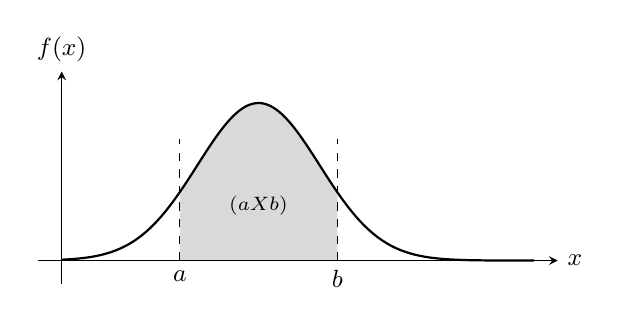
\begin{tikzpicture}[>=stealth, font=\small]
		\fill[black!15, domain=1.5:3.5, variable=\x] plot ({\x},{2*exp(-(\x-2.5)*(\x-2.5)/1.2)}) -- (3.5,0) -- (1.5,0) -- cycle;
		\draw[thick, domain=0:6, samples=100, smooth] plot (\x,{2*exp(-(\x-2.5)*(\x-2.5)/1.2)});
		\draw[->] (-0.3,0) -- (6.3,0) node[right] {$x$};
		\draw[->] (0,-0.3) -- (0,2.4) node[above] {$f(x)$};
		\draw[dashed] (1.5,0) -- (1.5,1.55);
		\draw[dashed] (3.5,0) -- (3.5,1.55);
		\node[below] at (1.5,0) {$a$};
		\node[below] at (3.5,0) {$b$};
		\node at (2.5,0.7) {\scriptsize $\Prob(a\leqslant X\leqslant b)$};
	\end{tikzpicture}
\end{center}

\begin{attention}
	Pour une variable continue, $\Prob(X=a)=0$ : les probabilités d'un point
	sont nulles. Ainsi $\Prob(a\leqslant X\leqslant b) = \Prob(a<X<b)$, et
	l'on peut passer librement de $<$ à $\leqslant$.
\end{attention}

\begin{remarque}
	L'\textbf{espérance} d'une variable continue de densité $f$ est
	$\Esp(X)=\displaystyle\int t\,f(t)\,\mathrm{d}t$ (intégrale sur
	l'intervalle où $f$ n'est pas nulle).
\end{remarque}


% ============================================================
\section{Loi uniforme}
% ============================================================

\begin{definition}[Loi uniforme]
	$X$ suit la \textbf{loi uniforme} sur $[a\,;b]$ lorsque sa densité est
	constante sur cet intervalle :
	$f(x) = \dfrac{1}{b-a}$ pour $x\in[a\,;b]$.
\end{definition}

\begin{center}
	\begin{tikzpicture}[>=stealth, font=\small]
		\draw[->] (-0.5,0) -- (5.5,0) node[right] {$x$};
		\draw[->] (0,-0.3) -- (0,2.2) node[above] {$f(x)$};
		\draw[thick] (0,0) -- (1,0) -- (1,1.5) -- (4,1.5) -- (4,0) -- (5,0);
		\draw[dashed] (0,1.5) -- (4,1.5);
		\node[left] at (0,1.5) {\small $\dfrac{1}{b-a}$};
		\node[below] at (1,0) {$a$};
		\node[below] at (4,0) {$b$};
	\end{tikzpicture}
\end{center}

\begin{propriete}{Loi uniforme}{prop_unif}
	Si $X$ suit la loi uniforme sur $[a\,;b]$, alors pour tout
	$[c\,;d]\subset[a\,;b]$ :
	\[
	\Prob(c\leqslant X\leqslant d) = \frac{d-c}{b-a},
	\qquad\text{et}\qquad
	\Esp(X) = \frac{a+b}{2}.
	\]
\end{propriete}


% ============================================================
\section{Loi exponentielle}
% ============================================================

\begin{definition}[Loi exponentielle]
	$X$ suit la \textbf{loi exponentielle} de paramètre $\lambda>0$ lorsque
	sa densité est $f(t) = \lambda\,\e^{-\lambda t}$ pour $t\geqslant 0$
	(et $f(t)=0$ pour $t<0$).
\end{definition}

\begin{center}
	\begin{tikzpicture}[>=stealth, font=\small]
		\draw[->] (-0.3,0) -- (5.5,0) node[right] {$t$};
		\draw[->] (0,-0.3) -- (0,2.5) node[above] {$f(t)$};
		\draw[thick, domain=0:5, samples=100, smooth] plot (\x,{2*exp(-\x)});
		\node[left] at (0,2) {$\lambda$};
	\end{tikzpicture}
\end{center}

\begin{propriete}{Loi exponentielle}{prop_exp}
	Si $X$ suit la loi exponentielle de paramètre $\lambda$, alors pour tout
	$t\geqslant0$ :
	\[
	\Prob(X\leqslant t) = 1-\e^{-\lambda t}, \qquad
	\Prob(X>t) = \e^{-\lambda t}, \qquad
	\Esp(X) = \frac{1}{\lambda}.
	\]
\end{propriete}

\begin{propriete}{Absence de mémoire}{prop_sansmemoire}
	Pour tous $s\geqslant 0$, $t\geqslant 0$ :
	\[
	\Prob_{X>s}(X>s+t) = \Prob(X>t).
	\]
	« Sachant qu'un composant a déjà duré $s$, la probabilité qu'il dure $t$
	de plus ne dépend pas de $s$. »
\end{propriete}

\begin{methode}
	\textbf{Preuve de l'absence de mémoire :}
	\[
	\Prob_{X>s}(X>s+t)
	= \frac{\Prob(X>s+t)}{\Prob(X>s)}
	= \frac{\e^{-\lambda(s+t)}}{\e^{-\lambda s}}
	= \e^{-\lambda t} = \Prob(X>t).
	\]
\end{methode}

\begin{exemple}
	La durée de vie (en années) d'un composant suit la loi exponentielle de
	paramètre $\lambda=0{,}1$. Alors
	$\Prob(X>5) = \e^{-0{,}5} \approx 0{,}607$, et l'espérance de durée de vie
	est $\dfrac{1}{0{,}1}=10$ ans.
\end{exemple}


% ============================================================
\section{Loi normale centrée réduite}
% ============================================================

\begin{definition}[Loi normale centrée réduite]
	$X$ suit la \textbf{loi normale centrée réduite} $\mathscr{N}(0,1)$
	lorsque sa densité est
	$f(t) = \dfrac{1}{\sqrt{2\pi}}\,\e^{-t^2/2}$ pour $t\in\R$.
	On note $\Phi(t)=\Prob(X\leqslant t)$ sa fonction de répartition.
\end{definition}

\begin{center}
	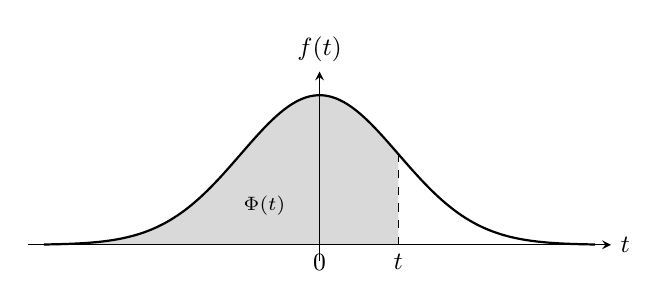
\begin{tikzpicture}[>=stealth, font=\small]
		\fill[black!15, domain=-3.5:1, variable=\x] plot ({\x},{1.9*exp(-\x*\x/2)}) -- (1,0) -- (-3.5,0) -- cycle;
		\draw[thick, domain=-3.5:3.5, samples=150, smooth] plot (\x,{1.9*exp(-\x*\x/2)});
		\draw[->] (-3.7,0) -- (3.7,0) node[right] {$t$};
		\draw[->] (0,-0.2) -- (0,2.2) node[above] {$f(t)$};
		\draw[dashed] (1,0) -- (1,1.15);
		\node[below] at (0,0) {$0$};
		\node[below] at (1,0) {$t$};
		\node at (-0.7,0.5) {\scriptsize $\Phi(t)$};
	\end{tikzpicture}
\end{center}

\begin{propriete}{Symétrie}{prop_sym}
	La courbe de $\mathscr{N}(0,1)$ est symétrique par rapport à l'axe des
	ordonnées. Pour tout réel $t$ :
	\[
	\Phi(-t) = 1-\Phi(t),\qquad
	\Prob(X\geqslant t) = 1-\Phi(t),
	\]
	\[
	\Prob(-t\leqslant X\leqslant t) = 2\Phi(t)-1.
	\]
\end{propriete}

\begin{astucebac}
	Les valeurs de $\Phi$ se lisent dans une \textbf{table de la loi normale}
	ou à la calculatrice. Quelques valeurs utiles :
	\begin{center}
	\begin{tabular}{|c|c|c|c|c|c|c|}
		\hline
		$t$ & $0{,}5$ & $1$ & $1{,}28$ & $1{,}5$ & $1{,}645$ & $1{,}96$ \\
		\hline
		$\Phi(t)$ & $0{,}691$ & $0{,}841$ & $0{,}900$ & $0{,}933$ &
		$0{,}950$ & $0{,}975$ \\
		\hline
	\end{tabular}
	\end{center}
	En particulier $\Prob(-1{,}96\leqslant X\leqslant 1{,}96)\approx 0{,}95$.
\end{astucebac}


% ============================================================
\section{Loi normale \texorpdfstring{$\mathscr{N}(m,\sigma^2)$}{N(m,sigma carre)}}
% ============================================================

\begin{definition}[Loi normale générale]
	$X$ suit la \textbf{loi normale} $\mathscr{N}(m,\sigma^2)$ (avec
	$\sigma>0$) lorsque la variable \textbf{centrée réduite}
	$Z = \dfrac{X-m}{\sigma}$ suit $\mathscr{N}(0,1)$. Alors $\Esp(X)=m$ et
	$\sigma(X)=\sigma$.
\end{definition}

\begin{methode}
	\textbf{Calculer $\Prob(a\leqslant X\leqslant b)$ pour
	$X\sim\mathscr{N}(m,\sigma^2)$ :} poser $Z=\dfrac{X-m}{\sigma}$, alors
	\[
	\Prob(a\leqslant X\leqslant b)
	= \Prob\!\left(\frac{a-m}{\sigma}\leqslant Z\leqslant\frac{b-m}{\sigma}\right)
	= \Phi\!\left(\frac{b-m}{\sigma}\right) - \Phi\!\left(\frac{a-m}{\sigma}\right).
	\]
\end{methode}

\begin{propriete}{Résultats à retenir (règle $68$–$95$–$99{,}7$)}{prop_regle}
	Si $X\sim\mathscr{N}(m,\sigma^2)$ :
	\[
	\Prob(m-\sigma\leqslant X\leqslant m+\sigma) \approx 0{,}6826,
	\]
	\[
	\Prob(m-2\sigma\leqslant X\leqslant m+2\sigma) \approx 0{,}9544,
	\]
	\[
	\Prob(m-3\sigma\leqslant X\leqslant m+3\sigma) \approx 0{,}9974.
	\]
\end{propriete}

\begin{center}
	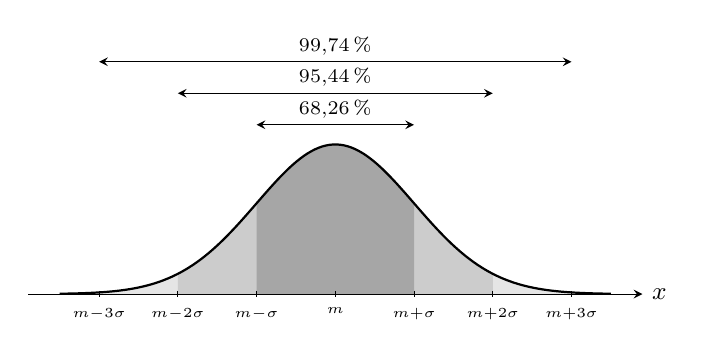
\begin{tikzpicture}[>=stealth, font=\small]
		\fill[black!10, domain=-3:3, variable=\x] plot ({\x},{1.9*exp(-\x*\x/2)}) -- (3,0) -- (-3,0) -- cycle;
		\fill[black!20, domain=-2:2, variable=\x] plot ({\x},{1.9*exp(-\x*\x/2)}) -- (2,0) -- (-2,0) -- cycle;
		\fill[black!35, domain=-1:1, variable=\x] plot ({\x},{1.9*exp(-\x*\x/2)}) -- (1,0) -- (-1,0) -- cycle;
		\draw[thick, domain=-3.5:3.5, samples=150, smooth] plot (\x,{1.9*exp(-\x*\x/2)});
		\draw[->] (-3.9,0) -- (3.9,0) node[right] {$x$};
		\foreach \x in {-3,-2,-1,0,1,2,3}{
			\draw (\x,0.04) -- (\x,-0.04);
		}
		\node[below] at (-3,-0.05) {\tiny $m{-}3\sigma$};
		\node[below] at (-2,-0.05) {\tiny $m{-}2\sigma$};
		\node[below] at (-1,-0.05) {\tiny $m{-}\sigma$};
		\node[below] at (0,-0.05) {\tiny $m$};
		\node[below] at (1,-0.05) {\tiny $m{+}\sigma$};
		\node[below] at (2,-0.05) {\tiny $m{+}2\sigma$};
		\node[below] at (3,-0.05) {\tiny $m{+}3\sigma$};
		\draw[<->] (-1,2.15) -- (1,2.15);
		\node at (0,2.35) {\scriptsize $68{,}26\,\%$};
		\draw[<->] (-2,2.55) -- (2,2.55);
		\node at (0,2.75) {\scriptsize $95{,}44\,\%$};
		\draw[<->] (-3,2.95) -- (3,2.95);
		\node at (0,3.15) {\scriptsize $99{,}74\,\%$};
	\end{tikzpicture}
\end{center}


% ============================================================
\section{Méthodes et exercices résolus}
% ============================================================

\begin{methode}
	\textbf{Trouver un seuil (quantile) :} pour déterminer $a$ tel que
	$\Prob(X\leqslant a)=\alpha$ avec $X\sim\mathscr{N}(m,\sigma^2)$ :
	\begin{enumerate}
		\item lire dans la table le réel $u$ tel que $\Phi(u)=\alpha$ ;
		\item résoudre $\dfrac{a-m}{\sigma}=u$, d'où $a = m+\sigma u$.
	\end{enumerate}
\end{methode}

\exerciceresolu
\textbf{Règle $68$–$95$–$99{,}7$}

Le poids $X$, en kg, des nouveau-nés d'une maternité suit
$\mathscr{N}(3{,}2\,;0{,}16)$.
\begin{enumerate}
	\item Préciser $m$ et $\sigma$.
	\item Calculer $\Prob(2{,}8\leqslant X\leqslant3{,}6)$.
	\item Calculer $\Prob(X\geqslant3{,}6)$.
\end{enumerate}

\solution

\textbf{1.} $m=3{,}2$ et $\sigma^2=0{,}16$, donc $\sigma=0{,}4$.

\textbf{2.} $2{,}8 = m-\sigma$ et $3{,}6 = m+\sigma$, donc
$\Prob(2{,}8\leqslant X\leqslant3{,}6) \approx 0{,}6826$.

\textbf{3.} Par symétrie autour de $m$ :
$\Prob(X\geqslant3{,}6) = \dfrac{1-0{,}6826}{2} \approx 0{,}1587$.

\exerciceresolu
\textbf{Standardisation}

Les notes $X$ d'un concours suivent $\mathscr{N}(10\,;9)$. On donne
$\Phi(1{,}5)\approx 0{,}933$ et $\Phi(1)\approx 0{,}841$.
\begin{enumerate}
	\item Calculer $\Prob(X\leqslant 14{,}5)$.
	\item Calculer $\Prob(7\leqslant X\leqslant 14{,}5)$.
	\item Déterminer la note $a$ telle que $10\,\%$ des candidats aient plus
	de $a$ (on donne $\Phi(1{,}28)\approx 0{,}9$).
\end{enumerate}

\solution

$m=10$, $\sigma=3$, $Z=\dfrac{X-10}{3}$.

\textbf{1.} $\Prob(X\leqslant 14{,}5)=\Phi\!\left(\dfrac{4{,}5}{3}\right)
=\Phi(1{,}5)\approx 0{,}933$.

\textbf{2.} $\Prob(7\leqslant X\leqslant 14{,}5)
=\Phi(1{,}5)-\Phi\!\left(\dfrac{-3}{3}\right)
=\Phi(1{,}5)-\bigl(1-\Phi(1)\bigr)
= 0{,}933-0{,}159 = 0{,}774$.

\textbf{3.} On veut $\Prob(X>a)=0{,}1$, soit $\Prob(X\leqslant a)=0{,}9$, donc
$\dfrac{a-10}{3}=1{,}28$ et $a = 10+3\times1{,}28 = 13{,}84$.

\exerciceresolu
\textbf{Loi exponentielle}

La durée $X$ (en heures) entre deux pannes d'un serveur suit la loi
exponentielle de paramètre $\lambda = 0{,}02$.
\begin{enumerate}
	\item Calculer $\Prob(X>50)$ et $\Prob(X\leqslant 100)$.
	\item Le serveur fonctionne depuis $30$ h. Calculer la probabilité qu'il
	tienne encore $50$ h.
	\item Donner la durée moyenne entre deux pannes.
\end{enumerate}

\solution

\textbf{1.} $\Prob(X>50)=\e^{-0{,}02\times 50}=\e^{-1}\approx 0{,}368$ ;
$\Prob(X\leqslant 100)=1-\e^{-2}\approx 0{,}865$.

\textbf{2.} Par absence de mémoire :
$\Prob_{X>30}(X>80)=\Prob(X>50)=\e^{-1}\approx 0{,}368$.

\textbf{3.} $\Esp(X)=\dfrac{1}{0{,}02}=50$ h.


% ============================================================
\section{Exercices d'entraînement}
% ============================================================

% --------------------------------------------------
\subsection{Échauffement}
% --------------------------------------------------

\exercice{Lire une aire \hfill \facile}
$X$ suit $\mathscr{N}(0,1)$. On donne $\Phi(1)\approx 0{,}841$ et
$\Phi(2)\approx 0{,}977$.
\begin{enumerate}
	\item Faire un schéma de la courbe et hachurer $\Prob(X\leqslant 1)$.
	\item Calculer $\Prob(X\geqslant 1)$ et $\Prob(-1\leqslant X\leqslant 1)$.
	\item Calculer $\Prob(X\leqslant -2)$.
\end{enumerate}

\exercice{Vrai ou faux \hfill \facile}
Répondre par \emph{vrai} ou \emph{faux} en justifiant.
\begin{enumerate}
	\item Pour une variable continue, $\Prob(X=3)=0$.
	\item Une densité de probabilité peut prendre des valeurs supérieures à
	$1$.
	\item Si $X$ suit la loi uniforme sur $[0\,;4]$, alors $\Esp(X)=2$.
	\item Pour la loi exponentielle, $\Prob(X>s+t)=\Prob(X>s)\Prob(X>t)$.
	\item La courbe de $\mathscr{N}(0,1)$ est symétrique par rapport à l'axe
	des ordonnées.
	\item Si $X\sim\mathscr{N}(m,\sigma^2)$, alors
	$\Prob(X\leqslant m)=\dfrac12$.
	\item $\Prob(m-2\sigma\leqslant X\leqslant m+2\sigma)\approx 0{,}95$.
\end{enumerate}

% --------------------------------------------------
\subsection{Lois uniforme et exponentielle}
% --------------------------------------------------

\exercice{Loi uniforme \hfill \facile}
Un bus passe toutes les $20$ min ; le temps d'attente $X$ suit la loi
uniforme sur $[0\,;20]$.
\begin{multicols}{2}
\begin{enumerate}
	\item Densité de $X$.
	\item $\Prob(X<5)$.
	\item $\Prob(8\leqslant X\leqslant 15)$.
	\item $\Esp(X)$.
\end{enumerate}
\end{multicols}

\exercice{Loi exponentielle \hfill \moyen}
La durée de vie $X$ (en heures) d'une ampoule suit la loi exponentielle de
paramètre $\lambda=0{,}002$.
\begin{enumerate}
	\item Calculer $\Prob(X>500)$ et $\Prob(X\leqslant 200)$.
	\item Donner la durée de vie moyenne.
	\item Sachant qu'elle fonctionne depuis $300$ h, calculer la probabilité
	qu'elle tienne encore $200$ h.
	\item Déterminer $t$ tel que $\Prob(X>t)=0{,}5$ (durée de vie médiane).
\end{enumerate}

% --------------------------------------------------
\subsection{Loi normale}
% --------------------------------------------------

\exercice{Règle empirique \hfill \facile}
$X\sim\mathscr{N}(12\,;4)$.
\begin{multicols}{2}
\begin{enumerate}
	\item Préciser $m$ et $\sigma$.
	\item $\Prob(8\leqslant X\leqslant 16)$.
	\item $\Prob(X\geqslant 16)$.
	\item $\Prob(X\leqslant 6)$.
\end{enumerate}
\end{multicols}

\exercice{Standardisation \hfill \moyen}
$X\sim\mathscr{N}(50\,;25)$. On donne $\Phi(0{,}8)\approx 0{,}788$,
$\Phi(1{,}4)\approx 0{,}919$.
\begin{enumerate}
	\item Calculer $\Prob(X\leqslant 54)$.
	\item Calculer $\Prob(43\leqslant X\leqslant 57)$.
	\item Déterminer $a$ tel que $\Prob(X\leqslant a)=0{,}919$.
\end{enumerate}

% --------------------------------------------------
\subsection{Sujets types Bac}
% --------------------------------------------------

\exercice{Sujet type Bac — masse de paquets \hfill \difficile}
Une machine remplit des paquets de riz dont la masse $X$ (en g) suit
$\mathscr{N}(1000\,;100)$.
\begin{enumerate}
	\item Préciser $m$ et $\sigma$.
	\item Un paquet est conforme si $980\leqslant X\leqslant 1020$. Sachant que
	$980 = m-2\sigma$ et $1020 = m+2\sigma$, calculer la probabilité qu'un
	paquet soit conforme.
	\item En déduire la probabilité qu'un paquet soit non conforme.
	\item Sur $500$ paquets produits, estimer le nombre de paquets non
	conformes.
	\item On donne $\Phi(1{,}5)\approx 0{,}933$. Calculer $\Prob(X\geqslant
	1015)$.
	\item On veut régler la machine (en changeant $\sigma$, à $m=1000$
	inchangé) pour que $99\,\%$ des paquets soient conformes. Sachant que
	$\Phi(2{,}575)\approx 0{,}995$, déterminer la valeur de $\sigma$
	convenable.
\end{enumerate}

\exercice{Sujet type Bac — durée de vie exponentielle \hfill \difficile}
La durée de vie $X$ (en années) d'un appareil suit la loi exponentielle de
paramètre $\lambda>0$. Une étude donne $\Prob(X>4)=0{,}55$.

\textbf{Partie A}
\begin{enumerate}
	\item Exprimer $\Prob(X>4)$ en fonction de $\lambda$ et en déduire
	$\lambda = \dfrac{-\ln 0{,}55}{4}$ ; en donner une valeur approchée.
	\item Calculer la durée de vie moyenne de l'appareil.
	\item Calculer $\Prob(X\leqslant 2)$.
\end{enumerate}

\textbf{Partie B}
\begin{enumerate}
	\setcounter{enumi}{3}
	\item Un appareil a déjà fonctionné $6$ ans. Calculer la probabilité
	qu'il fonctionne encore $4$ ans.
	\item Déterminer la durée $t$ telle que $\Prob(X\leqslant t)=0{,}5$
	(médiane).
	\item Un lot contient $10$ appareils identiques et indépendants. En
	utilisant $\Prob(X>4)=0{,}55$, calculer la probabilité qu'au moins un
	appareil dépasse $4$ ans.
\end{enumerate}

\exercice{Sujet type Bac — temps d'attente \hfill \difficile}
À un guichet, le temps de service $X$ (en minutes) suit la loi uniforme sur
$[2\,;10]$.
\begin{enumerate}
	\item Donner la densité de $X$ et calculer $\Esp(X)$.
	\item Calculer $\Prob(X\leqslant 5)$ et $\Prob(X\geqslant 8)$.
	\item Calculer $\Prob(4\leqslant X\leqslant 7)$.
	\item Sachant que le service a déjà duré $6$ minutes, calculer la
	probabilité qu'il dure au total moins de $8$ minutes.
	\item Trois clients sont servis successivement et indépendamment.
	Calculer la probabilité que les trois services durent chacun moins de
	$5$ minutes.
\end{enumerate}

\exercice{Sujet type Bac — notes d'examen \hfill \difficile}
Les notes $X$ à un examen suivent $\mathscr{N}(11\,;9)$. On donne
$\Phi(1)\approx 0{,}841$, $\Phi(1{,}28)\approx 0{,}900$,
$\Phi(1{,}645)\approx 0{,}950$.

\textbf{Partie A}
\begin{enumerate}
	\item Préciser $m$ et $\sigma$.
	\item Calculer la proportion de candidats ayant au moins $14$
	($X\geqslant 14$).
	\item Calculer $\Prob(8\leqslant X\leqslant 14)$.
\end{enumerate}

\textbf{Partie B}
\begin{enumerate}
	\setcounter{enumi}{3}
	\item On attribue une mention aux $10\,\%$ meilleurs. Déterminer la note
	minimale pour l'obtenir.
	\item On élimine les $5\,\%$ plus faibles. Déterminer la note en dessous
	de laquelle on est éliminé.
	\item Sur $400$ candidats, estimer le nombre de mentions.
\end{enumerate}

\exercice{Sujet type Bac — contrôle d'un réglage \hfill \difficile}
Une machine découpe des tiges dont la longueur $X$ (en mm) suit
$\mathscr{N}(m\,;\sigma^2)$. Le cahier des charges impose
$99\,\%$ des tiges dans l'intervalle $[298\,;302]$.
\begin{enumerate}
	\item On admet que la production est centrée : $m = 300$. Traduire la
	condition sur $\sigma$ à l'aide de la variable $Z = \dfrac{X-300}{\sigma}$.
	\item Sachant que $\Prob(-u\leqslant Z\leqslant u)=0{,}99$ pour
	$u\approx 2{,}575$, déterminer la plus grande valeur de $\sigma$
	acceptable.
	\item Avec $\sigma = 0{,}8$ mm, calculer $\Prob(X<298)$ (on donne
	$\Phi(2{,}5)\approx 0{,}994$).
	\item Sur $1000$ tiges, estimer le nombre de tiges hors norme.
\end{enumerate}
